\section{Foundations}
\label{sec:foundations}

The previous section positioned open-vocabulary and reasoning segmentation as a convergence of dense prediction, vision-language representation, promptable mask generation, and multimodal reasoning. This section defines the reusable components behind that convergence. We first introduce the common notation for images, language queries, features, masks, and vocabularies. We then summarize the foundation components that recur across later method sections, including CLIP-style encoders, SAM/SAM2-style mask generators, grounding modules, and MLLM-based reasoning interfaces. Finally, we review the main learning objectives and evaluation setups used to compare these systems.

\subsection{Visual, textual, and mask representations}

Let $I \in \mathbb{R}^{H \times W \times 3}$ denote an input image and $q$ denote a language input. Depending on the task, $q$ can be a category name, a prompted label set $\mathcal{C}=\{c_1,\ldots,c_N\}$, a referring expression, an instruction, or a multi-turn dialogue. A vision-language segmentation system typically maps $I$ to dense visual features $F=\phi_I(I)\in\mathbb{R}^{h\times w\times d}$ and maps text to embeddings $T=\{\phi_T(c_i)\}_{i=1}^{N}$ or to an instruction embedding $\phi_T(q)$. Closed-set segmentation learns a fixed classifier over $\mathcal{C}$, whereas open-vocabulary segmentation replaces or augments that classifier with text-derived embeddings so that new categories can be introduced at inference time~\citep{radford2021learning,liang2023ovseg,xshanOpenvocabularySemanticSegmentation2024}.

This formulation creates three common representation levels. The first is the pixel or patch level, where each spatial feature $f_u$ is compared with text embeddings and assigned a semantic label. A simple open-vocabulary prediction rule is
\begin{equation}
    \hat{y}_u = \arg\max_{c_i \in \mathcal{C}} \; \operatorname{sim}(f_u,t_i),
\end{equation}
where $\operatorname{sim}(\cdot,\cdot)$ is usually cosine similarity after normalization. This level is natural for semantic segmentation, but it inherits the mismatch between image-level vision-language pre-training and localized pixel semantics. Recent dense alignment methods therefore refine patch-text or pixel-text correspondence rather than directly applying global image-text features to segmentation~\citep{yangExploringCLIPsDense2025,yxchngAligningVisionLanguageModel2026}.

The second level is the region or mask level. A mask generator produces candidate masks $\mathcal{M}=\{m_k\}_{k=1}^{K}$, and each mask is represented by a pooled region feature
\begin{equation}
    r_k = \operatorname{Pool}(F,m_k).
\end{equation}
The system then classifies, ranks, or grounds masks by comparing $r_k$ with text embeddings. This formulation supports proposal-then-classification and mask-text alignment pipelines, where the spatial problem and the semantic problem are partially decoupled. Universal segment embeddings, SAM-assisted open-vocabulary segmentation, and mask-adapted CLIP methods follow this logic by treating masks as the basic recognition unit rather than predicting labels independently for all pixels~\citep{xwangUseUniversalSegment2024,kirillov2023sam,xhanBoostingSegmentAnything2025,lee2025escnet}.

The third level is the token level used by grounded and reasoning segmentation. Instead of only producing a mask or a class name, the model may generate a textual response containing grounding tokens, segmentation tokens, coordinates, or references to masks. LISA introduces a segmentation token interface for reasoning segmentation, PixelLM uses pixel-level localization inside a language-model framework, and GLaMM grounds generated conversational responses with segmentation masks~\citep{xlaiLisaReasoningSegmentation2024,renPixellmPixelReasoning2024,rasheedGlammPixelGrounding2024}. This level is essential when the target is implicit: the model must first infer what should be segmented and then bind the inferred answer to pixels.

\begin{figure*}[t]
    \centering
    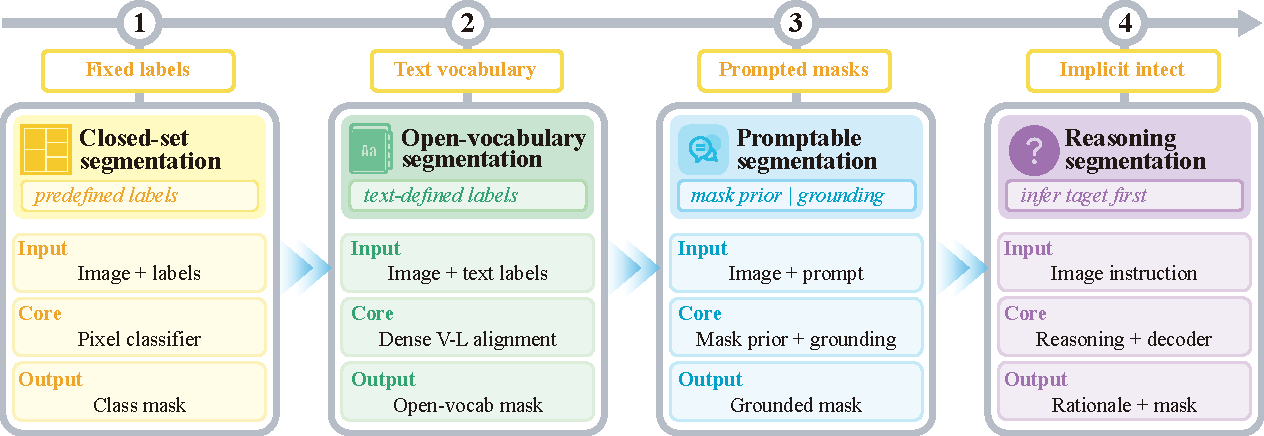
\includegraphics[width=0.98\textwidth]{Fig/foundation_paradigms.pdf}
    \caption{Four foundation paradigms used in this survey. Closed-set segmentation fixes the label space; open-vocabulary segmentation introduces text-defined categories; promptable and grounded segmentation combines reusable mask priors with language grounding; reasoning segmentation adds an inference stage before mask generation.}
    \label{fig:foundation_paradigms}
\end{figure*}

Fig.~\ref{fig:foundation_paradigms} summarizes the role of these representation levels. The later taxonomy can be read as a gradual increase in interface flexibility: from fixed class labels, to text-defined vocabularies, to promptable masks, and finally to instructions whose target must be reasoned out before segmentation.

\subsection{Foundation components}

\textbf{Vision-language encoders.} CLIP-style dual encoders provide the basic semantic space for many open-vocabulary segmentation methods. The image encoder produces global or patch-level visual features, the text encoder embeds class names or prompts, and recognition is performed by measuring image-text similarity~\citep{radford2021learning}. For segmentation, the key issue is not whether CLIP recognizes an image-level concept, but whether its features preserve spatially reliable semantics. This motivates mask-adapted CLIP, side adapters, label-free dense transfer, patch-text calibration, and fine-grained semantic reconstruction methods that adapt global image-text knowledge to dense prediction~\citep{liang2023ovseg,xu2023san,luo2024pnpovss,yangExploringCLIPsDense2025,yxchngAligningVisionLanguageModel2026}.

\textbf{Mask generators and decoders.} SAM-style segmentation foundation models provide strong class-agnostic mask priors through prompt encoders and mask decoders~\citep{kirillov2023sam}. In open-vocabulary and grounded segmentation, SAM is rarely the whole solution because it does not by itself assign open semantic labels. Its value lies in producing high-quality spatial candidates that can be classified, filtered, or grounded by vision-language modules. Recent SAM/SAM2-based methods therefore integrate mask proposals with open-vocabulary detectors, lightweight VLM embeddings, language prompts, or universal segmentation objectives~\citep{xhanBoostingSegmentAnything2025,hwangXSAMSegmentAnything2026,sgxiaoOpenworldsamExtendingSam22026,shinhOpenvocabularySemanticSegmentation2024}. This component explains why many methods report strong boundary quality while still requiring careful semantic calibration.

\textbf{Grounding modules.} Grounding modules bind language units to regions, masks, or spatial coordinates. In referring expression segmentation, the input is usually a phrase or sentence and the output is the corresponding mask. In grounded multimodal conversation, generated words or object mentions can be linked to masks. Region-word grounding and mask-text alignment are therefore intermediate mechanisms between open-vocabulary category recognition and reasoning segmentation. Pixel-aligned language models, LLaVA-Grounding, Ferret, OneRef, and GLaMM illustrate different ways to represent regions, words, masks, and generated responses in a shared grounding interface~\citep{xuPixelalignedLanguageModel2024,zhangLlavagroundingGroundedVisual2024,youFerretReferGround2024,xiaoOnerefUnifiedOnetower2024,rasheedGlammPixelGrounding2024}.

\textbf{MLLM reasoners and segmentation heads.} Reasoning segmentation adds a language-model reasoning component to the mask pipeline. One design inserts a segmentation token into an MLLM and decodes masks from the hidden state of that token, as in LISA-style systems~\citep{xlaiLisaReasoningSegmentation2024}. Another design uses a pixel decoder or segmentation expert to convert language-model decisions into masks, as in PixelLM, GLaMM, and later MLLM-guided segmentation systems~\citep{renPixellmPixelReasoning2024,rasheedGlammPixelGrounding2024,zhangOmgllavaBridgingImagelevel2024}. A third design decomposes reasoning and perception by using external detectors, segmenters, or agents to iteratively select candidate regions~\citep{luoConnectingDotsTrainingFree2026,huangPixelsLogicPerceptionReasoning2026}. These designs differ in where the mask is produced, but they share the same requirement: the textual rationale and the spatial mask must refer to the same visual evidence.

\subsection{Learning and adaptation objectives}

The first family of objectives is dense image-text alignment. A common contrastive form compares visual features and text features in a shared embedding space:
\begin{equation}
    \mathcal{L}_{\mathrm{itc}} =
    -\frac{1}{B}\sum_{i=1}^{B}
    \log
    \frac{\exp(\operatorname{sim}(v_i,t_i)/\tau)}
    {\sum_{j=1}^{B}\exp(\operatorname{sim}(v_i,t_j)/\tau)} ,
\end{equation}
where $v_i$ and $t_i$ are matched visual and textual embeddings and $\tau$ is a temperature parameter. For segmentation, $v_i$ may correspond to a patch, a region, or a mask rather than an entire image. Pixel-aligned contrastive learning and dense CLIP adaptation use this principle to improve local semantic transfer~\citep{sikdarPicazoPixelalignedContrastive2025,yangExploringCLIPsDense2025}. The strength of this objective is vocabulary transfer; its limitation is that similarity scores can be poorly calibrated across categories, domains, or mask granularities.

The second family is region-word and mask-text alignment. These objectives supervise the correspondence between a word or phrase and a spatial unit, often through matching losses, contrastive ranking, cross-attention, or mask classification. They are especially important for referring expression segmentation and grounded conversation, where a phrase may describe attributes, relations, or fine-grained parts rather than a single class name. Works such as PixelLM, LLaVA-Grounding, OneRef, and GLaMM show that mask-aware alignment can turn language from a label source into a grounding interface~\citep{xuPixelalignedLanguageModel2024,zhangLlavagroundingGroundedVisual2024,xiaoOnerefUnifiedOnetower2024,rasheedGlammPixelGrounding2024}.

The third family covers lightweight adaptation and distillation. Prompt learning, adapters, side networks, mask adapters, and feature calibration modules try to preserve foundation-model knowledge while adding dense prediction ability. Distillation transfers semantics from VLMs, SAM, DINO-like vision models, or task specialists into a segmentation model when dense labels are scarce. This family is prominent because open-vocabulary segmentation often cannot afford full retraining on exhaustive pixel labels. However, adaptation objectives must be interpreted together with their supervision source: image-level labels, pseudo masks, class names, prompt-generated masks, and domain-specific weak labels create different failure modes~\citep{xu2023san,shinhOpenvocabularySemanticSegmentation2024,libExploringEfficientOpenvocabulary2026}.

The fourth family is instruction tuning, RL, and preference optimization for reasoning-to-mask systems. Supervised instruction tuning teaches the MLLM to follow segmentation-oriented prompts and emit mask-related tokens or grounded responses. RL and preference optimization then optimize properties that are difficult to express with token-level likelihood alone, such as reasoning format, visual faithfulness, spatial accuracy, and hallucination avoidance. Recent work uses reward-guided or preference-based training to improve chain-of-thought segmentation, task alignment, affordance grounding, medical grounding, and implicit reasoning segmentation~\citep{yanTaskPreferenceOptimization2025,zhuLensLearningSegment2026,zhouReasoningImplicitSelfsupervised2026,yanMedreasonerReinforcementLearning2026,wangAffordancer1ReinforcementLearning2026}. These objectives are promising, but they make evaluation more complex because a model can improve its language format without improving mask quality unless rewards explicitly measure visual grounding.

\subsection{Evaluation setups}

Open-vocabulary evaluation usually asks whether a method can segment categories that were not densely annotated during training. The key variants are zero-shot evaluation, where the test vocabulary is provided only through text; generalized open-vocabulary evaluation, where base and novel categories are evaluated together; and domain-transfer evaluation, where the target images come from a different distribution such as remote sensing or medical imagery. Meaningful comparison requires reporting the backbone, training data, vocabulary construction, prompt templates, and whether the method uses target-domain images or labels~\citep{hhuangRenovatingNamesOpenvocabulary2024,libExploringEfficientOpenvocabulary2026}.

Promptable and grounded evaluation changes the unit of comparison from category labels to prompts and language-region correspondences. A point, box, mask, category name, phrase, or sentence can lead to different candidate masks and different ambiguity. Referring expression segmentation commonly evaluates mask overlap for sentence-level references, while grounded conversation also evaluates whether generated object mentions are linked to correct regions. For this reason, mask quality alone is insufficient: the benchmark must specify prompt type, target granularity, whether multiple regions can be valid, and how ungrounded or over-grounded language is penalized~\citep{youFerretReferGround2024,rasheedGlammPixelGrounding2024,huGroundingSuiteMeasuringComplex2025}.

Reasoning segmentation evaluation adds another layer. The query may require commonsense, spatial inference, guideline following, or task-specific rules before a mask can be produced. The evaluation must therefore consider at least three outputs: the inferred target, the textual rationale or response, and the final mask. Recent benchmarks and methods expose this issue by testing implicit instructions, false premises, rich context, multi-agent refinement, video reasoning, 3D referring, medical reasoning, affordance grounding, and remote-sensing transfer~\citep{guoSeeingBelievingRichContext2026,vvatsGuidelineConsistentSegmentationMultiAgent2026,xuVideosegr1ReasoningVideo2026,chen3DDRESDetailed3D2026,yanMedreasonerReinforcementLearning2026,wangAffordancer1ReinforcementLearning2026}. In later sections, we use this foundation to separate improvements in semantic openness, spatial precision, promptability, and reasoning faithfulness rather than treating all gains as the same type of progress.
